
\chapter[Implementation]{Implementation}
\graphicspath{ {images/implementation} }
In this chapter, we present how we designed and implemented SYN, a tool that supports the software evolution comprehension approach 
defined in section \ref{s:EvolutionModel} and \ref{s:3DRepr}. 

% In section x we provide an overview of our platform by looking at all the modules that compose the architecture. 
% In section x we present the user interface of the tool and finally in section x we detail how we implemented the auditory part. 


\section{Platform overview}

SYN is a platform tool that allows developers to have a visual and auditive depiction of an evolving system. 
It was designed to be extensible and efficient, therefore, we created a set of modules each one with its own responsibility:
\begin{itemize}
    \item \textbf{SYN Core}: the core module, required by other modules. It holds the core concepts of SYN, such as ProjectHistories, ProjectVersions, and so on. It also provides some abstract concepts that are open to any kind of implementation to achieve the extensibility goal.
    \item \textbf{SYN CLI}: responsible to provide a Command Line Interface interaction to users.
    \item \textbf{SYN Analyzer}: implements the analysis approach described in section \ref{s:EvolutionModel}. 
    \item \textbf{SYN Server}: provides GraphQL endpoints to retrieve data from SYN and display them in a user interface. 
    \item \textbf{SYN Debugger}: the user interface of SYN developed to debug and visually depict information collected during the analysis. 
\end{itemize}

All the modules of SYN are written in Java with the exception of SYN Debugger which is written with React and TypeScript. 

The modular architecture of SYN allows the user to interact with the tool in two different ways: through the console with the commands provided by the SYN CLI module 
or through a web application embedded inside the SYN Debugger module. \\
Figure \ref{fig:architecture} provides an high-level overview of the architecture. Each row represents the dependencies between modules.
The heart of the system is the SYN Core module. 
It specifies concepts described in out approach and it also standardize how modules should interact with it.
It holds a View Generator used by other components to create views over the collected repository's data. 
This collection is done by the SYN Analyzer module, internally, it has classes that act as a repository explorer to retrieve data from the repositotory history. 
Moreover, metrics are extracted with the metrics extractor component and put inside the internal historical representation trought the history builder component. 
Since we wanted to provide a direct access to the analysis capabilities of SYN, the SYN CLI priovides commands that directly calls functions defined inside SYN Analyzer. 
This is the reason why it has both SYN Core and SYN Analyzer as dependencies. 

SYN Debugger holds the GUI of SYN to graphically represent a view. Information are retrived through endpoints specified by the GraphQL server of the SYN Server module, that, in turn, retrieves view data from the SYN Core module. 


\begin{figure}
    \center
    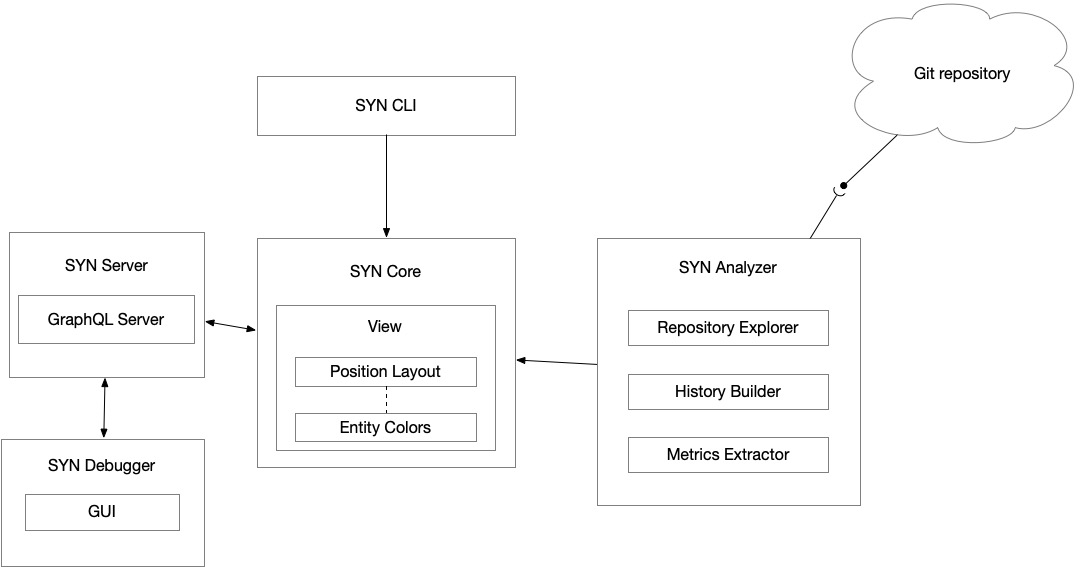
\includegraphics[width=\textwidth]{SYNArchitecture.jpg}
    \caption{Architecture of SYN}
    \label{fig:architecture}
\end{figure}

Having reached a low coupling between modules, the extennsibility of SYN is preserved. In fact, modules such as the server or the analysis implementation could be changed without altering the codebase of other modules. 

\section{SYN Core}
SYN Core is a module that holds all the entities that we have introduced in section \ref{s:EvolutionModel}. 
All the classes of our model, extend the \texttt{Entity} class that is composed of the field \texttt{id}, which is unique and is used to identify an object inside our domain. 
To quickly identify the type of the object, each class has an identifier that makes the prefix of the id. 
Classes inside the model of SYN Core could be partitioned into four subdomains: Project, History, Analysis, and View. 

\subsection*{Project}
The fist part of the model consists of the \textbf{Project} entities. 
The diagram is shown in image \ref{fig:modelProject}. The abstract class \texttt{Project} represents a software system. It defines the following fields:
\begin{itemize}
    \item \textbf{name}: the name of the project.
    \item \textbf{projectHistory}: an object that represents the history of the project. It holds the results of the analysis. 
    \item \textbf{path}: the path of the git repository. 
\end{itemize}

Moreover, we defined two additional classes \texttt{LocalProject} and \texttt{RemoteProject} that respectively represent a project that was already cloned and present in the local storage and a project that needs to be retrieved from the internet. 
Therefore, if on one hand, \texttt{LocalProject} does not need any further fields to represent a local project on the other hand \texttt{RemoteProject} needs at least the \texttt{projectURL} field. We might add more information such as the git branch, and the remote credentials but we decided to keep the implementation as simple as possible. 

\texttt{LocalProject}

\begin{figure}
    \center
    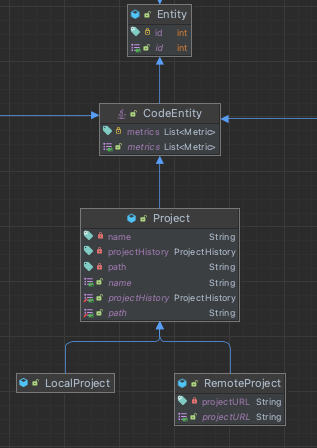
\includegraphics[width=0.2\textwidth]{UMLProject.png}
    \caption{Model: Project entities}
    \label{fig:modelProject}
\end{figure}

\subsection*{History}

\begin{figure}
    \center
    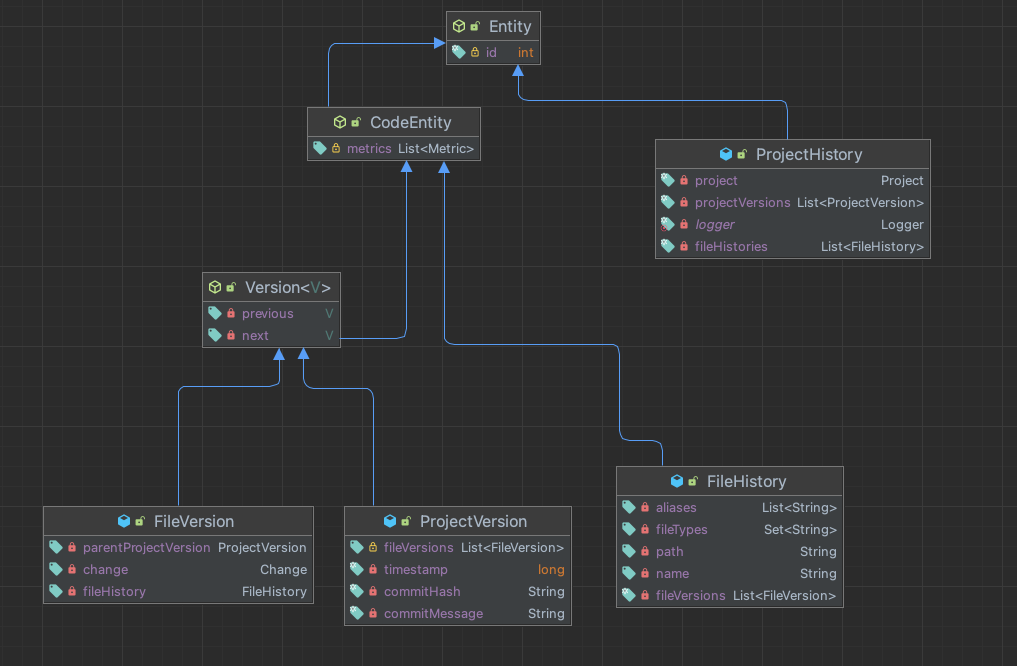
\includegraphics[width=0.2\textwidth]{UMLHistory.png}
    \caption{Model: History entities}
    \label{fig:modelHistory}
\end{figure}

As we evidenced above, each project might hold \textbf{ProjectHistory} object that represents its history. 
Following what we have explained in section \ref{s:EvolutionModel}, the ProctHistory class holds a group of ProjectVersion and a group of FileHistories. The FileHistory class, which represents the history of a single file, consists of:
\begin{itemize}
    \item aliases: a list of paths related to the file. We know that a file is identified by a single unique name. However, since our approach is tolerant to moving and renaming activities, we have to store somewhere all the paths that a file had. In section X we explain the importance of this field and why it has such a crucial role in our analysis. 
    \item fileTypes: A set of Strings each one representing the type of this file. 
    \item Path: the path of the file.
    \item Name: the name of the file.
    \item fileVersions: a list of FileVersions related to this fileHistory. 
\end{itemize}
With the \texttt{VersionV} class we want to represent the state of an entity at a particular point in time. 
The generic parameter \texttt{V} is used as a constraint to force a consistency of the type of the previous and the next version. 
The \texttt{ProjectVersion} class, used to represent git commits, defines the following fields: 
\begin{itemize}
    \item fileVersions: a list of FileVerions that are part of this commit.
    \item timestamp: The timestamp of the commit. 
    \item commitHash: the hash of the commit. 
    \item commitMessage: the message of the commit.
\end{itemize}
Extending the Version class, the ProjectVersion class inherits also the previous and next field that could be used to traverse the history similar to how we traverse a LinkedList. 
Finally, the \texttt{FileVersion} class has the following fields:
\begin{itemize}
    \item parentProjectVersion: the ProjectVersion holding this FileVersion instance. It can be used to retrieve the commit's related information such as the timestamp or the message. 
    \item change: an object that represents the action made on that file. 
    \item fileHistory: the FileHistory that represents the file being modified. 
\end{itemize}

A change represents an action made on a file. In our approach, we have identified five different types of changes, and in our implementation, all of them extend the \texttt{Change} class. It is composed of the field \texttt{linesAdded} and \texttt{linesRemoved} each one representing the number of lines added and removed. 
The goal of our model is to be easily extensible. With that in mind, if in a future implementation we want to extend the variety of metrics specifically collected for each kind of change, we just need to extend the relative class and the polymorphic mechanisms of Java will do the rest. 

\begin{figure}
    \center
    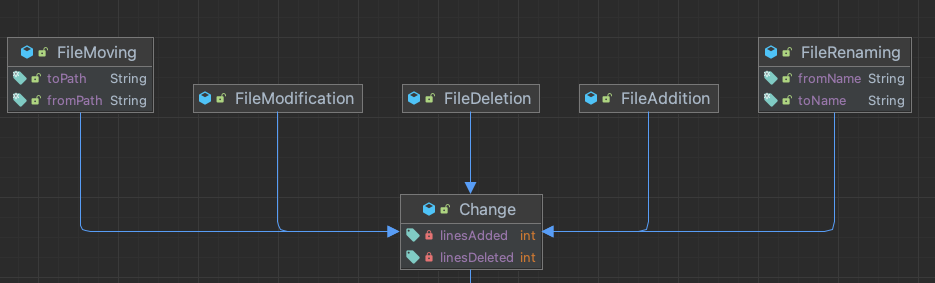
\includegraphics[width=0.5\textwidth]{UMLChanges.png}
    \caption{Model: Change entities}
    \label{fig:modelChange}
\end{figure}


\subsection*{Analysis}
Even though the analysis is effectively implemented into another module, SYN Core provides some abstract classes that need to be implemented to allow the exchange of analysis results. 
The first class that the model defines is \textbf{AnalysisWorkDescriptor}.
An AnalysisWorkDescriptor is, as the name suggests, a holder of useful information to instruct the analyzer on what it has to do. This information comprehends the project on which we have to run the analysis and the list of commits that have to be analyzed. 
The reasons behind this implementation choice are to allow multiple threads to run in parallel multiple analyses without analyzing the same commit multiple times. 
We described this approach in section \ref{s:partialHistoricalRepr}.
\bigbreak

Inside the core module we also have the \textbf{FileTypeManager} class. Its responsibility is to map a set of function to compute evolutionary metrics, (presented in section \ref{s:evolutionaryMetrics}) given a fileHistory. The returned set of functions could be easily extended also with external modules. This choice was made to easily allow external components to increase the set of metrics computed in SYN. In fact, we allow any developer to write any kind of function able to compute any kind of metric and put it inside the set of the corresponding file type. 
We can easily infer the implications of this design, for example, if in the future an engineer wants to write an OO (Object Oriented) metric, such as the number of parents, they can create a function to compute that and associate that function to the "JAVA" or the "OO" type. 
\bigbreak

Finally, in our model, we also defined the \textbf{ProjectAnalysisResult} class. It must be used by an analyzer to return the results that it collected. Moreover, this class made a distinction between partial and total analysis results, allowing it to be used with the partial history retrival approach defined in section \ref{s:partialHistoricalRepr}. The fields declared on this class are:
\begin{itemize}
    \item project: the projects on which the analysis was done.
    \item analysisCompleted: whether if the analysis is partial or total.
    \item timestamp: the timestamp of the moment when the analysis was completed. 
    \item firstCommit: the first commit considered in this analysis. 
    \item lastCommit: the last commit considered in this analysis. 
    \item projectVersions: a list of ProjectVersion discovered during the analysis.
    \item fileHistories: a list of FileHistories discovered during the analysis.
    \item fileVersions: a list of FileVersions discovered during the analysis.
\end{itemize}

Moreover, this module also provides an abstraction of the core concepts of the Git protocol. The classes are \texttt{GitProject}, \texttt{GitCommit} and \texttt{GitChange} each one respectively representing a repository, a commit and a change on a a file. 
With this choice each external module has an high level of autonomy, having the possibility to decide how it should interact with git. 

\subsection*{View}
\label{s:view_impl}
The concept of View in SYN is related to how information should be displayed. In section \ref{s:3DRepr} explained our visual approach. To implement it, we have defined a class called \textbf{View}, that designates how the visualuaziation should be rendered. 
In our visualization approach, we have to display the evolution of a repository. To do that the user interface needs to sequentially display one by one a list of frames, each one representing a moment of the repository. A moment could be either a group of commits in space or a group of commits in time.
We designed the class \textbf{ViewAnimation} to represent a frame of the evolutionary animation of the view. This class has two properties:
\begin{itemize}
    \item \texttt{representedEntities}: a list of ProjectVersions whose data had been used to create that frame.
    \item \texttt{viewFigureList}: a list of ViewFigure each one representing a FileHistory in the view.
\end{itemize}

The \textbf{ViewFigure} class holds graphical properties to properly display each FileHistory
\begin{itemize}
    \item \texttt{position}: the position of the entity.
    \item \texttt{color}: the color of the entity.
    \item \texttt{height}: the height of the entity.
    \item \texttt{shape}: a literal that represents the shape of the entity. 
    \item \texttt{age}: the age of the entity.
    \item \texttt{enabled}: wether the enity should be visualized or not.
    \item \texttt{opacity}: the opacity of the entity.
    \item \texttt{size}: the size of the entity.
\end{itemize}

All these properties are computed when the \texttt{View} object is instantiated. A view is created on the top of the user's preferences. 
So, for example, if the user wants to use a specific color for a specific action, like the dark green for the additions, we have to store this information somewhere. 
This is the reason why we defined the \textbf{ViewSpecification} class. A \texttt{View Specification} is the key element of each view. 
All the views are generated from a \texttt{ViewSpecification} instance. The list of available properties defined inside a \texttt{ViewSpecification} are:
\begin{itemize}
    \item \texttt{versionGroupingStrategy}: the strategy that SYN needs to follow to group up commits and create moments.
    \item \texttt{versionGroupingChunkSize}: the dimension of each group; it can be a number of commits or an amount of time. 
    \item \texttt{colorPalette}: the mapping that SYN has to follow to map FileVersion's actions to colors. 
    \item \texttt{agingGroupingStrategy}: the strategy that SYN needs to follow to define an age.
    \item \texttt{agingStepSize}: the dimension of each age; it can be a number of commits or an amount of time. 
    \item \texttt{agingSteps}: the number of available aging steps. 
    \item \texttt{mapperStrategy}: the strategy that SYN has to follow to compute the height of each entity.
    \item \texttt{mapperStrategyOptions}: optional properties of the mapper if needed.
    \item \texttt{mapperMetricName}: the metric that the mapper should consider to compute the height. 
    \item \texttt{showUnmappedEntities}: wether the view should display entities without the selected metric.
    \item \texttt{fileTypeShape}: the mapping that SYN has to follow to associate a FileType with a shape.
    \item \texttt{fileTypeOpacity}: the mapping that SYN has to follow to associate a FileType with an opacity level.
    \item \texttt{figureSize}: the size of each figure.
    \item \texttt{figureSpacing}: the space between each figure.
    \item \texttt{showDeletedEntities}: wether the view should display deleted eneitites.
    \item \texttt{withGround}: wether the view should include a ground element.
\end{itemize}

Moreover, we defined an abstract class \textbf{PositionLayout} whose implementation specifies how entities should be laid out and a class \textbf{MapperStrategy} whose implementation specifies how the height of the entity is computed. With SYN we ship five possible mapperStrategy:
\begin{itemize}
    \item BucketCountStrategy: where the height of the entity is computed after performing a bucketing on the selected metric's values. 
    \item LinearBucketValueStrategy: where the height of the entity is computed after performing first a bucketing and then a linear mapping on the selected metric's values. 
    \item LinearMapperStrategy: where the height of the entity is computed after performing a linear mapping on the selected metric's values. 
    \item NormalizerMapperStrategy: where the height of the entity is computed after performing a normalization on the selected metric's values. 
\end{itemize}



\section{SYN CLI}
SYN CLI is a command-line interface that allows developers to interact with SYN. It gives to developers full control over the system.
\bigbreak
\textbf{Analysis commands}
\bigbreak

\lstinline{syn analyze auto -p <project_id> -o <output_file> -t <thread_count>}\\
\\
This command is used to run an automatic analysis with SYN. 
Given the id of the project, the system automatically creates all the thread workers (5 by default), runs in parallel the analysis, and joins the results in the output file. 
Moreover, this command ensures that each thread has its own git repository. 
\bigbreak

\lstinline{syn analyze join -o <output_file> <...analysis_file>}\\
\\
This command is used to join analysis results into a single output file.
\bigbreak
\begin{lstlisting}
syn analyze manual -p <project_id> -g <git_repo_path>
    -rc <first_commit> -lc <last_commit> -o <output_file>
\end{lstlisting}
\bigbreak
This command is used to perform a manual analysis with SYN. This command lets the developer have the freedom to choose the repository path and both the first and the last commit of the analysis. 
If the first commit is not specified the analysis starts from the beginning of the history and, in the same way, if the last commit is not specified the analysis ends with the end of the history. 
\bigbreak

\begin{lstlisting}
syn analyze prepare -p <project_id>  -g <git_repo_path> 
    -wn <workers_number> -of <output_folder>
\end{lstlisting}
\bigbreak
This command is used to create a folder of workers to analyze a project.
Based on the number of workers, the repository history is equally partitioned into chunks, and each one is assigned to a worker. 
\bigbreak

\lstinline{syn analyze worker -p <project_id> -g <git_repo_path> -w <worker_file -o <output_file>}\\
\\
This command is used to run the analysis on a project given its worker file. 
Moreover, here the user can specify the git path because it cannot be used by two analyzers at the same time, so it is up to the user to choose a free git repository. 

\bigbreak
\textbf{Prioject commands}
\bigbreak

\lstinline{syn project list}\\
\\
This command is used to print in the console a list of available projects

\bigbreak
\lstinline{syn project create -n <project_name> -p <project_location>}\\
\\
This command is used to create a project given its name and its location. The location could be either a path or an URL. 

\bigbreak
\lstinline{syn project inspect -g <git_path> <project_id> <FileHistory_id>}\\
\\
This command is used to inspect all the FileVersions of a FileHistory. Moreover, if the git repository is provided, SYN performs a double check to ensure that all the FileVersions were spotted. \
To do so, it exploits the output of the command "\lstinline{git log --full-history -- <FileHistory_path>}", keeping attention if the FileHistory's path was changed (git cannot do that).

\bigbreak
\lstinline{syn util csv <project_id> -o <output_file>}\\
\\
This command produces a CSV containing all the commit's tracked information of the selected project. 


\section{SYN Analyzer}
SYN Analyzer is a module that provides an implementation of the analysis approach described in section \ref{s:EvolutionModel}.
To walk through the git-tree, it uses a Java git adapter called JGit. 
To do so, we designed three subclasses of the SYN Core git classes, \texttt{JGitProject}, \texttt{JGitCommit} and \texttt{JGitChange}, that calls the JGit API to retrieve historical information. 
\bigbreak

To run the analysis we need to obtain first an \texttt{AnalysisWorkDescriptor}. 
In this modules, we developed a class \texttt{JGitAnalysisWorkerDescriptorFactory} to partition the commit tree and obtain a set of workers. 
Figure \ref{fig:historysplit} shows an example of a partition with 3 workers. First, the whole history of git is retrieved and stored in memory. Secondly, all the commits from all the branches are merged into a single list sorted by their timestamp. 
Then, the merge commits are removed since the changes recored by them are duplicated and finally the resulting list is partitioned to match the requested number of workers. 
\begin{figure}
    \center
    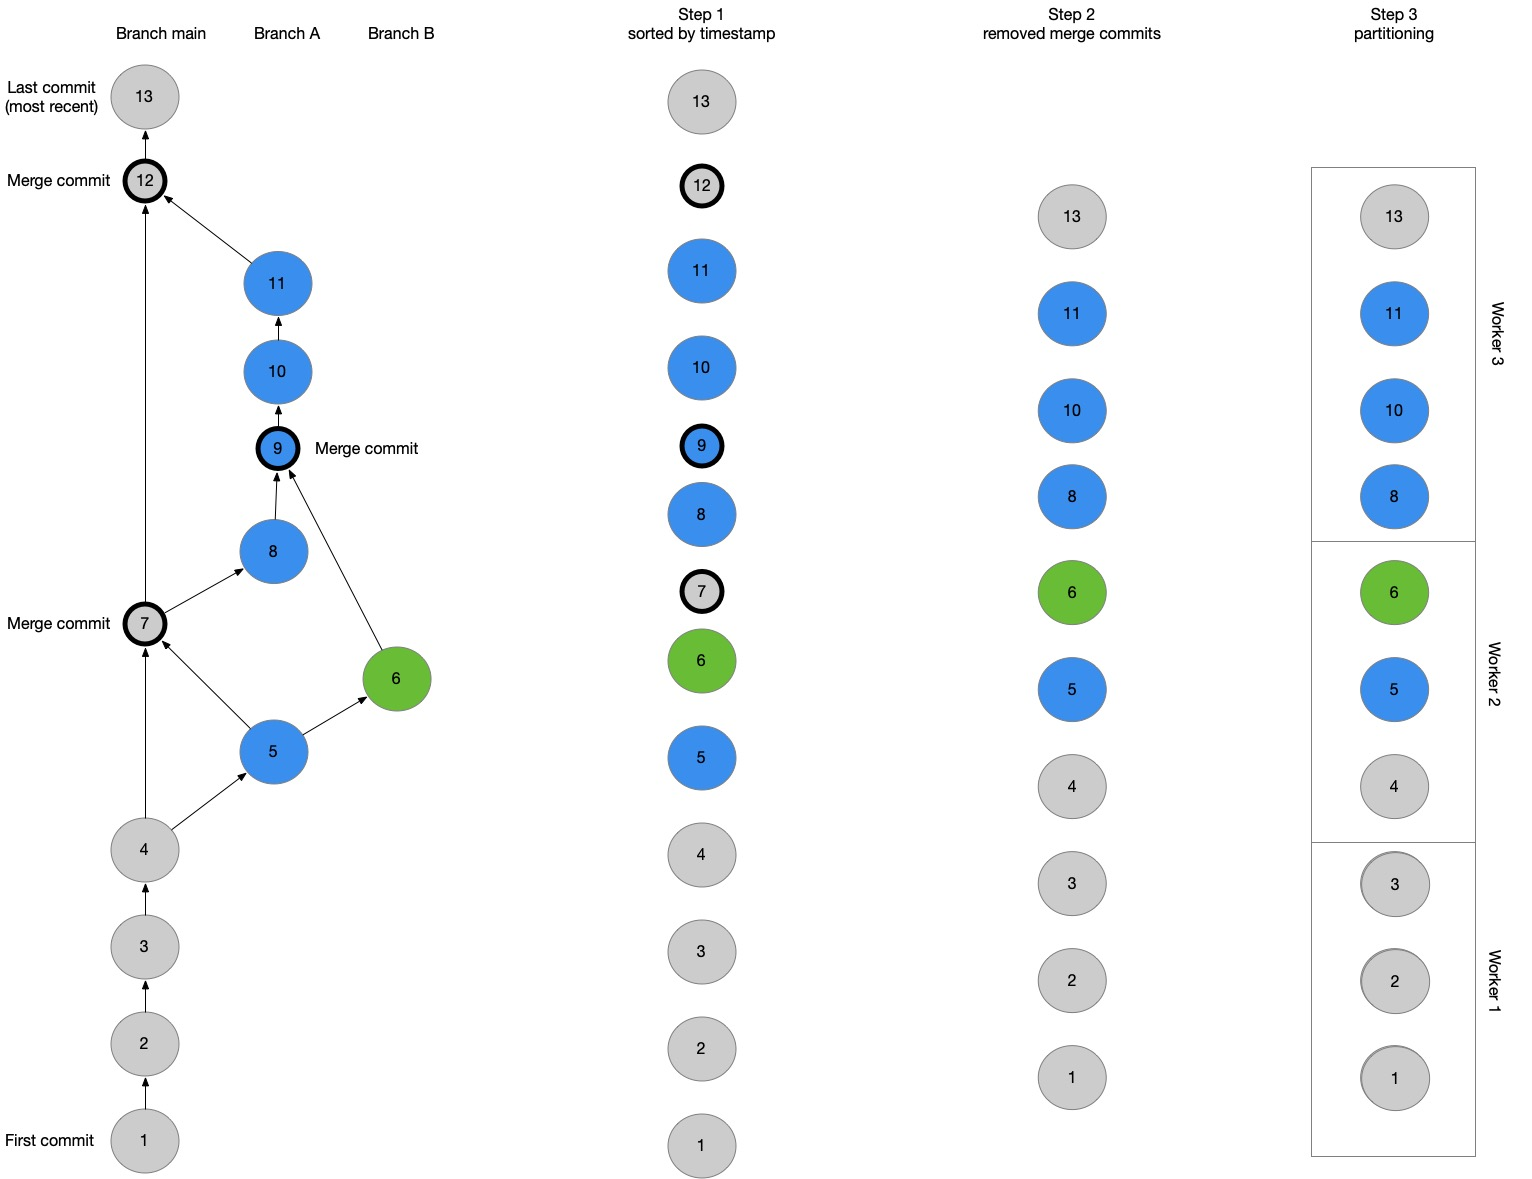
\includegraphics[width=\textwidth]{HistorySplit.jpg}
    \caption{Partition of the commit tree with 3 workers.}
    \label{fig:historysplit}
\end{figure}


The analysis process of a single worker contemplates the following steps:
\begin{enumerate}
    \item we call the method \texttt{runAnalysis} of the class \texttt{ProjectAnalyzer} with a worker descriptor and a project as an argument. 
    \item the analyzer reads the git path of the project and instantates a new \texttt{GitProject}. 
    \item a list of commits, specified in the worker, is retrieved from the \texttt{GitProject}.
    \item the first commit of the list is retrieved, a new \texttt{ProjectVersion} is created with its details. 
    \item the analyzer runs the checkout command of git to restore the version of the system at the one specified by the commit. 
    \item the analyzer retrieves a list of modified files. 
    \item for each modified file, the analyzer creates a new \texttt{FileVersion}, links it with the corresponding  \texttt{ProjectVersion} and \texttt{FileHistory} (creates it if it doesn't not exist yet), and finally extracts all the evolutionary metrics expected for that kind of file.
    \item one all the modified files are analyzed, and the analyzer repeats steps 5, 6, and 7 considering, each time the subsequent commit of the list. 
    \item one all the commits are analyzed, and the analyzer returns all the discovered results within an \texttt{ProjectAnalysisResult} object. 
\end{enumerate}

\bigbreak
If we want to analyze a large repository in an acceptable amount of time, we have to run the analysis in parallel and thus we have to use a considerable amount of workers. 
Each worker produces a \texttt{ProjectAnalysisResult}, then to obtain the full history of the repository we have to all the analysis results. 
In SYN each entity is identified by an id. 
The order in which entities are created is important because we visually sort entities based on their creation timestamp. 
Therefore, having consistency between ids of FileHistory is the most important feature that our algorithm must-have.
We said that each analysis result has: a list of \texttt{FileVersions}, a list of \texttt{ProjectVersions} and a list of \texttt{FileHistories}. 
Analyzers are not able to communicate, therefore each one works in a sandbox. 
When we have to join them, concatenating two lists of \texttt{FileVersions} or two lists of \texttt{ProjectVersions} is not a problem if the historical sequence was respected. 
In fact, these objects are mutually independent of each other.
The challenge comes with \texttt{FileHistories}. When the analyzer encour a file, if it was not discovered yet, it creates a new \texttt{FileHistory} with a new id. 
This sounds like a problem with merging because we might append the same file twice. In other words, we have an issue with linking FileHistories between analysis results.
Assuming for a moment that we do not have this obstacle, there is another situation that might happen, more tricky than the previous one. 
If in the middle of two analysis results a file changed its path, on the first analysis we have an entity with the old path, 
and on the second analysis, we have an entity with a new path. 
Unless we won't keep track of all the possible paths of an entity, it is impossible to reconstruct a connection between these two files. 
This is the reason that brought us to put the alias field in the \texttt{FileHistory} class. 

In the join algorithm that we developed, we employ a map to keep track of FileHistories.
As a result, nevertheless, the file has a different id on any analysis result, the consistency between
FileHistories is guaranteed and moreover, we can guarantee the absence of duplicates inside the newly built repository history. 

Therefore, the algorithm takes as input a list of already discovered FileHistories and an \texttt{ProjectAnalysisResult} and it returns a dictionary.
This dictionary is used to map partialFileHistories, the FileHistory of an analysis result, to definitiveFileHistories, which are part of the full history of the repository. 
To obtain this map it uses the following strategy:
\begin{enumerate}
    \item If the last alias of a definitiveFileHistories is equal to the first alias of a partialFileHistory then they represent the same file.
    \item If in the partialAnalysisResult there is more than one FileHistory with the same first alias, only the first is mapped to a definitiveFileHistories and the other partialAnalysisResult are mapped to a new newFileHistory.
    \item If a partialFileHistory has not an alias match with a previously created definitiveFileHistories then it represents a new definitiveFileHistories.
\end{enumerate}

% \begin{algorithm}
%     \caption{Algorithm to create a mapping between partialFileHistories and definitiveFileHistories}
%     \label{alg:cap}
%     \begin{algorithmic}[1]
        
%     \State $partialToDefinitiveMap \gets new Map()$
%     \State $partialAliasToFileHistory \gets new Map()$
%     \State $newFileHistories \gets new List()$
%     \end{algorithmic}
% \end{algorithm}

\begin{algorithm}
    \caption{Algorithm to create a mapping between partialFileHistories and definitiveFileHistories}\label{euclid}
    \begin{algorithmic}[1]
    \Procedure{PartialToDefinitiveFH}{$projectAnalysisResult, partialFileHistories$}
        \State $partialToDefinitive \gets Map()$
        \State $partialAliasToFH \gets Map()$ \Comment{Strategy 1}
        \State $unmappedPartialFileHistories \gets List()$  \Comment{Strategy 2}
        \ForAll{partialFH in partialFileHistories}
            \State $firstAlias \gets partialFH.aliases[0]$
            \If{$!partialAliasToFH.has(firstAlias)$}
                \State $partialAliasToFH.set(firstAlias, partialFH)$  \Comment{Strategy 1}
            \Else
                \State $unmappedPartialFH.append(partialAliasToFH)$  \Comment{Strategy 2}
            \EndIf
        \EndFor

        \ForAll{definitiveFH in projectAnalysisResult} \Comment{Strategy 1}
            \State $lastAlias \gets definitiveFH.aliases[definitiveFH.length - 1]$
            \If{$partialAliasToFH.has(lastAlias)$}
                \State $partialFH = partialAliasToFH.get(lastAlias)$
                \State $definitiveFH.path = partialFH.path$
                \State $definitiveFH.aliases.addAll(partialFH.aliases)$
                \State $partialToDefinitive.set(partialFH, definitiveFH)$
                \State $partialAliasToFH.remove(lastAlias)$
            \EndIf
        \EndFor

        \State $unmappedPartialFH.addAll(partialAliasToFH)$ \Comment{Strategy 3}
        \ForAll{partialFH in unmappedPartialFH} 
            \State $definitiveFH = FileHistory(partial.name, partial.path)$
            \State $definitiveFH.aliases = partialFH.aliases $
            \State $partialToDefinitive.set(partialFH, definitiveFH)$
        \EndFor
        \State \textbf{return} $partialToDefinitive$
    \EndProcedure
    \end{algorithmic}
\end{algorithm}


\section{SYN Server}
SYN Server is responsible for providing the elaborated information, given by the analysis results, in an intermediate language between the 
front-end (SYN Debugger) and the back-end. We used SpringBoot, a Spring-based tool for developing "production-ready" applications efficiently.

\subsection*{GraphQL API} 
This type of communication is used in SYN for retrieving repository information.
GraphQL is a query language for APIs that gives clients the possibility to ask for exactly what they need.
This is an advantage compared to a REST API because, instead of always returning a predefined set of data, with GraphQL only the needed information will be returned making the communication more effective. 
In GraphQL endpoints are divided into queries and mutations. Queries are used to retrieve data while mutations are used to create or alter data. 

\bigbreak
\textbf{Mutations}

=> \texttt{createProject(projectName: String!, projectLocation: String!): Project} 
used to create and automatically analyze a new project.
It takes as parameters the name of the project and its location (the path on the local machine or the URL), both as a String. 

\bigbreak
\textbf{Queries}

\texttt{projectList:  [PartialProjectInformation]!} \\ 
is used to retrieve a list of projects. For performance reasons, with this query only the name and the id of a project can be retrieved. 
\bigbreak
\texttt{view(projectId: Int!, viewSpecification: ViewSpecificationInput!): View} \\
returns a view of the project identified by the argument \texttt{projectId}, built following the directives specified in the \texttt{viewSpecification} object. 
This query returns an object representing a view, thus it has all the fields that we have described in section \ref{s:view_impl}. 
\bigbreak
\texttt{partialView(projectId: Int!, viewSpecification: ViewSpecificationInput!, viewAnimationId: Int): View} \\
returns a view with only the next 100 animations starting from the one identified by \texttt{viewAnimationId}. 
This endpoint was created to enable performance optimizations on clients. If the viewSpecification expected too many animations, the resulting view would be a bottleneck for the client.
With this endpoint it can still retrieve the view, and then animation can be lazily loaded once they are effectively required. 
\bigbreak
\texttt{fileHistory(projectId: Int!, fileHistoryId: Int!): FileHistory} \\
used to retrieve details of the FileHistory identified with \texttt{fileHistoryId} of the project identified with \texttt{projectId}.
\bigbreak
\texttt{projectVersions(projectId: Int!, projectVersionsId: [Int]!): [ProjectVersion]!} \\
used to retrieve details of the ProjectVersion identified with \texttt{projectVersionsId} of the project identified with \texttt{projectId}.
\bigbreak
\texttt{groupingPreview(projectId: Int!, viewSpecification: ViewSpecificationInput!): Int} \\
this endpoint is used to compute the number of AnimationFrames that are gonna be created with the given \texttt{viewSpecification}.
\bigbreak
\texttt{fileTypeCounter(projectId: Int!): [FileTypeCounter!]!} \\
this endpoint returns a list that maps each FileType with the number of occurrences that it has in the project \texttt{projectId}.
\bigbreak
\texttt{fileTypeMetrics(projectId: Int!, fileTypeFilter: [String]): [FileTypeMetrics!]!} \\
this endpoint returns a list that maps each FileType with a list of metrics available for it. Only the FileTypes specified in the \texttt{fileTypeFilter} list are considered. 


\section{SYN Debugger}

SYN Debugger is a web application that allows developers to interact with SYN. It is written with React.js, a popular JavaScript framework. 
The aim of this application is to have a visual depiction of the view generated by the server, plus some additional information. 
For example, it allows you to ckick on an entity and sees the information that is related to it. 
The visualization is based on Babylon.js, a popular 3D library. 
SYN Debugger provides a different kinds of customizations to the view, such as the shape and the colors of the entities. 
All these customizations are sent to the back-end server, through a {\em view specification} file. 

The main purpose of this application is to debug the view and explore all the possible visualization combinations of a system.
The main page of the visualization is a list of project.

\subsection*{Project setup}
Once a project is selected, the UI searches in the local storage of the web browser a view specification. 
If it is not present, the first view loaded is the project setup.
The project setup is a view that allows the user to express preferences about how the UI should be rendered. 
There are five steps that composes this view:
\begin{itemize}
    \item Component selection: where the user can express which kind of FileType must be considered in the viewSpecification. 
    To ease the choice, for each FileType a counter representing how many FileHistories have that FiltType is shown. 
    \item Grouping version strategy: enables the user to chose how moments should be created.
    \item Figure settings: to customize shape, metrics and opacity of each FileType. Moreover, with this view the user can chose the mapping strategy for the height of entities. 
    \item View color: to customize the color of each change and how aging must act. 
    \item View settings: to customize some general settings such as the speed of the visualization, shadows or wether deleted entities should be kept. 
\end{itemize}

\subsubsection*{Component selection}
The first step of the setup, shown in figure \ref{fig:SYNUIsettings1}, shows a list of cards, each one representing a FileType. 
We can break the visualization area into two parts: on the top one, there are two cartds to represent binary files and text files. 
The sum of this two counters represent the total number of FileHistories present in the system because each file must be textual or binary. 
On the bottom area there are all the cards whose type is extracted by the extension of the FileHistory. For example, is a file is named "foo.java" it is represented by the JAVA card in this area. 
Cards are sorted in a descending order by their counter. This views considers all the FileType present in the system, to show the complete list users has to click on the button "show more".

\begin{figure}
    \center
    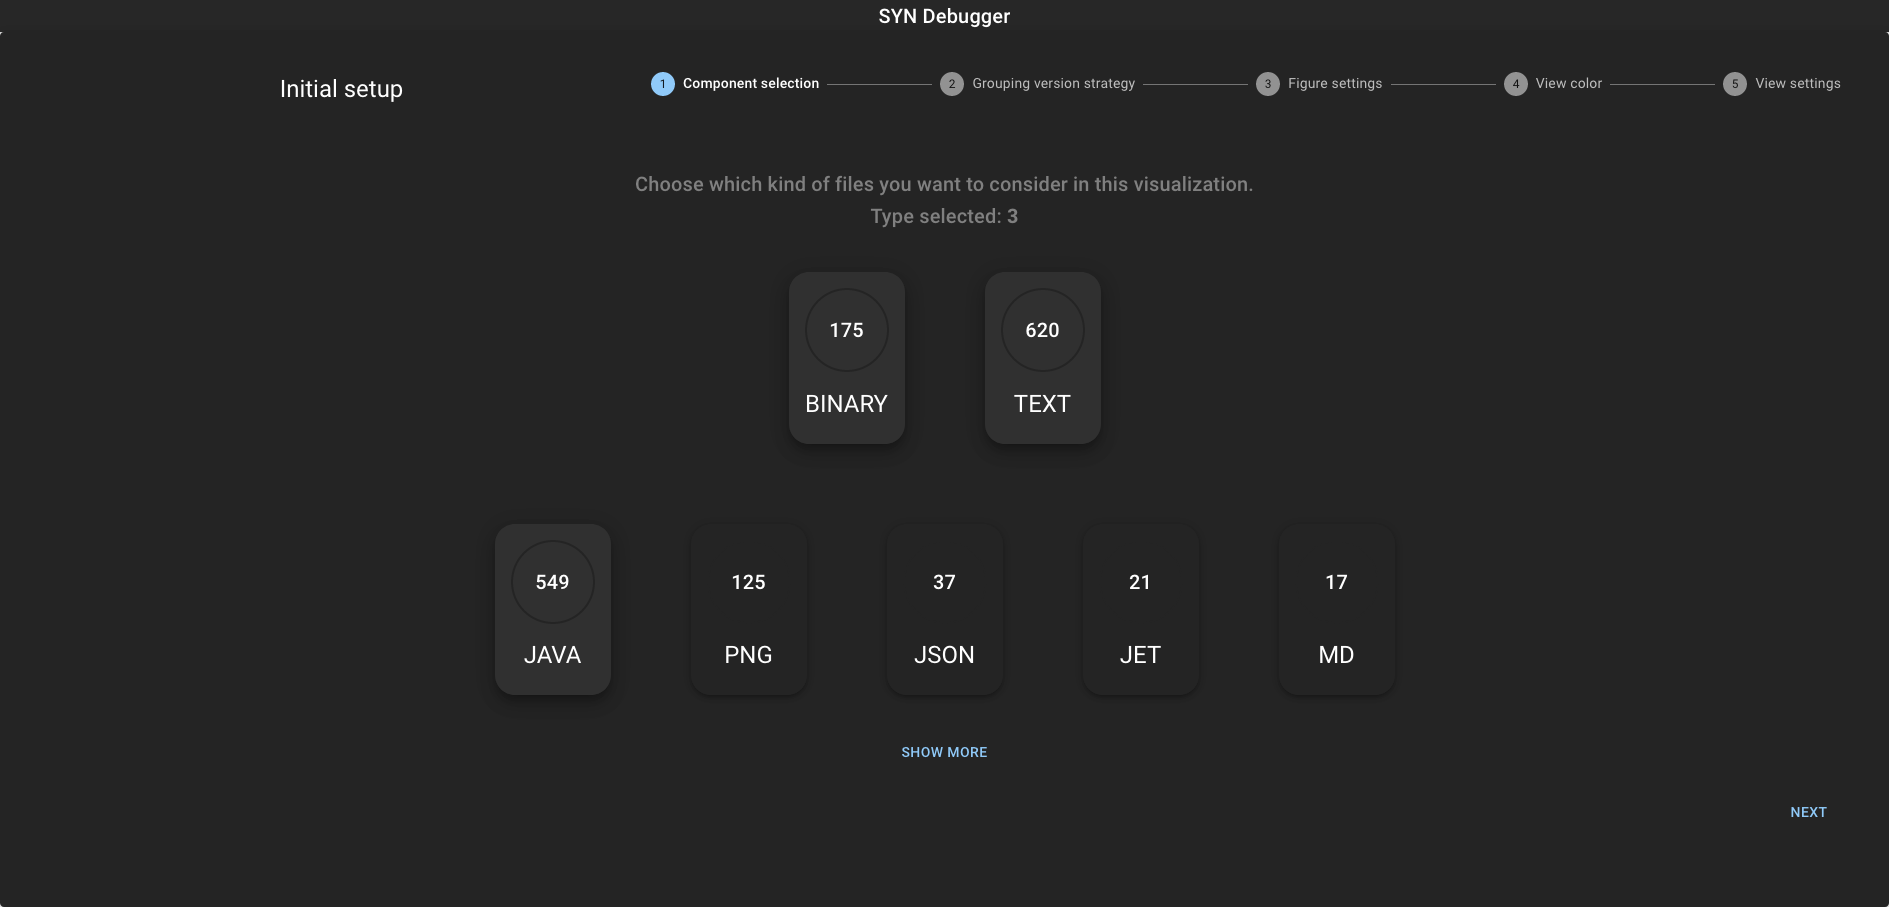
\includegraphics[width=\textwidth]{SYNUI-settings1.png}
    \caption{Project setup: component selection}
    \label{fig:SYNUIsettings1}
\end{figure}


\subsubsection*{Grouping strategy}
The second step of the setup, shown in figure \ref{fig:SYNUIsettings2}, allows the user to chose how SYN groups ProjectVersions. 
Following what we have presented in the visual approach section \ref{s:3DRepr}, we provide two strategies to group ProjectVersions:
\begin{itemize}
    \item by commits: we create a moment every $n$ commits. 
    \item by timestamp: we create a moment every $n$ seconds. 
\end{itemize}

To ease the selection of the timestamp strategy, instead of manually compute the width of the time window, the user has only to specify an amount and its time measure (hour, day, week, month, year) and the UI automatically does the rest. 
Moreover, the UI shows a preview of the grouping strategy to give an idea on how many animations are created with the selected settings. 
\begin{figure}
    \center
    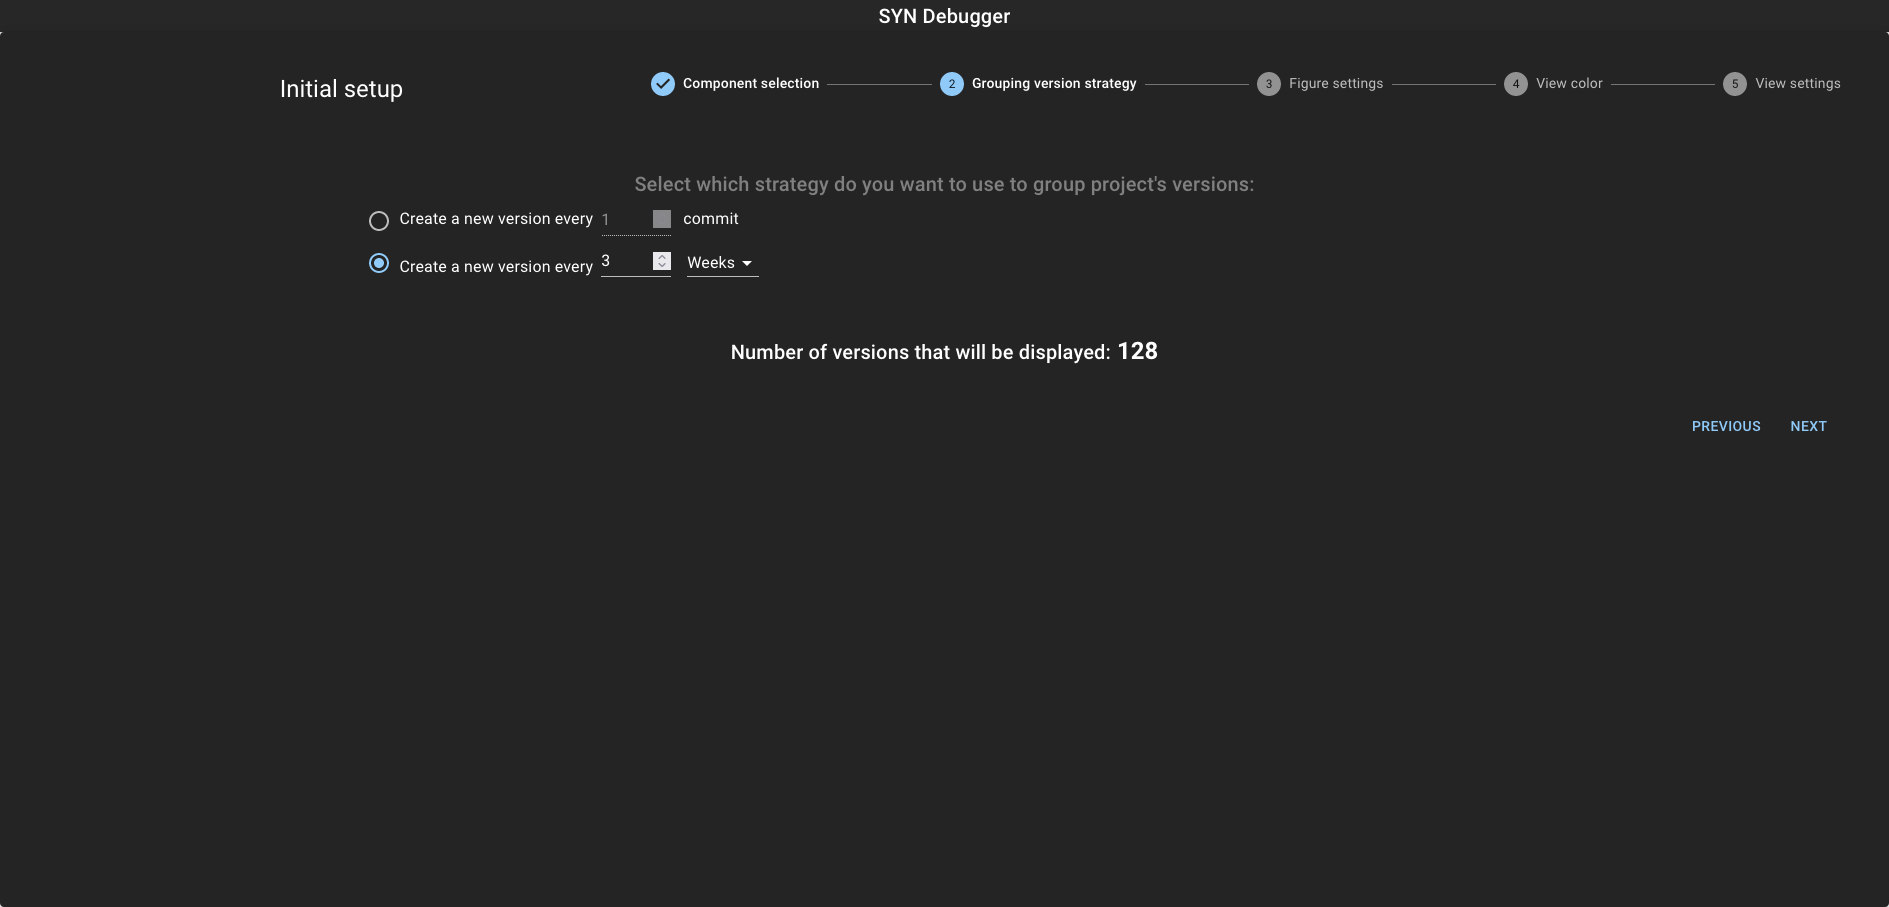
\includegraphics[width=\textwidth]{SYNUI-settings2.png}
    \caption{Project setup: grouping strategy}
    \label{fig:SYNUIsettings2}
\end{figure}

\subsubsection*{Figure settings}
The third step of the setup, shown in figure \ref{fig:SYNUIsettings3}, allows the user to express graphical preferences. 
For each FileType selected in the step "Component selection", a card is created in this view. 
On each card user can customize:
\begin{itemize}
    \item which metrics should be considered by the visualization. These metrics are displayed when an entity is selected.
    \item the shape of the entity in the visualization. In our visualization we implemented five kinds of shapes: BOX, TRIANGULAR, CONE, SPHERE and CYLINDER. 
    \item the opacity of each FileType. 
\end{itemize}

Moreover, the user can also express their preferences to chose which mapper strategies SYN has to use to compute the height of entities, which metric must be used by the mapper and the maximum height of the entities. 
The list of available metrics for the mapper, is composed by the metrics selected for each FileType.
As a consequence, the UI has a checkbox to specify wether FileHistories that do not have the selected metric, should be rendered or not. 
\bigbreak
With all the settings available on this page the user has the full control about how FileHistories are rendered. 
There are a lot of possible combinations, each one with its own purpose. For example, if we want a visualization that has a focus only on Java files, we can use the following settings:
\begin{itemize}
    \item BINARY metrics: none, shape: SPHERE, opacity: 0.3
    \item TEXT metrics: none, shape: SPHERE, opacity: 0.3
    \item JAVA metrics: SLOC, shape: BOX, opacity: 1
\end{itemize}
and for the mapper use the LinearBucketValueStrategy, with the SLOC metric and a maximum height of 20. 

\begin{figure}
    \center
    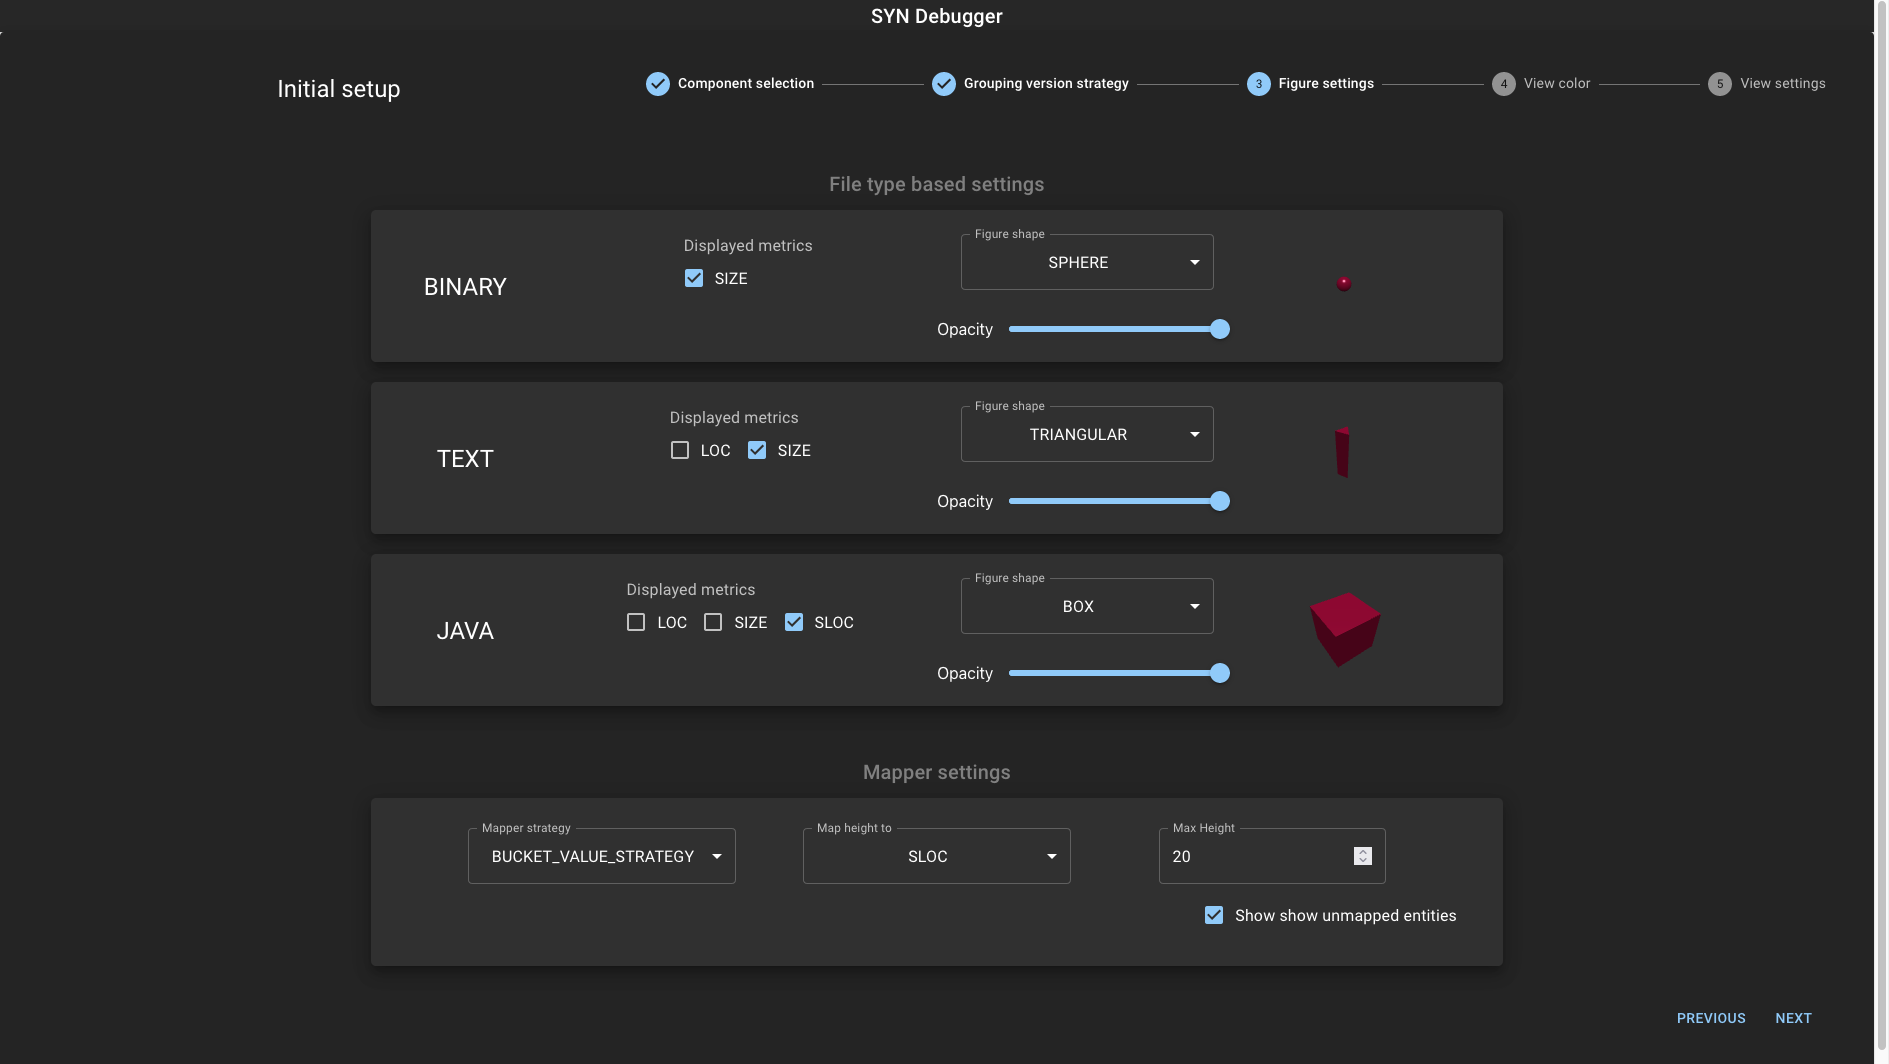
\includegraphics[width=\textwidth]{SYNUI-settings3.png}
    \caption{Project setup: figure settings}
    \label{fig:SYNUIsettings3}
\end{figure}

\subsubsection*{View color}
The fourth step of the setup, shown in figure \ref{fig:SYNUIsettings4}, allows the user to express preferences about the color mapping of entities. 

The user has the full control over the way how aging is computed. 
As with grouping versions, aging can be done following two possible strategies: one by timestamp and one by commits. 
The color transition is linear, therefore the user can choose the number of steps between the original color of the entity and the base color. 

Finally, each action has a distinct original color, that can be customized by the user. 

\begin{figure}
    \center
    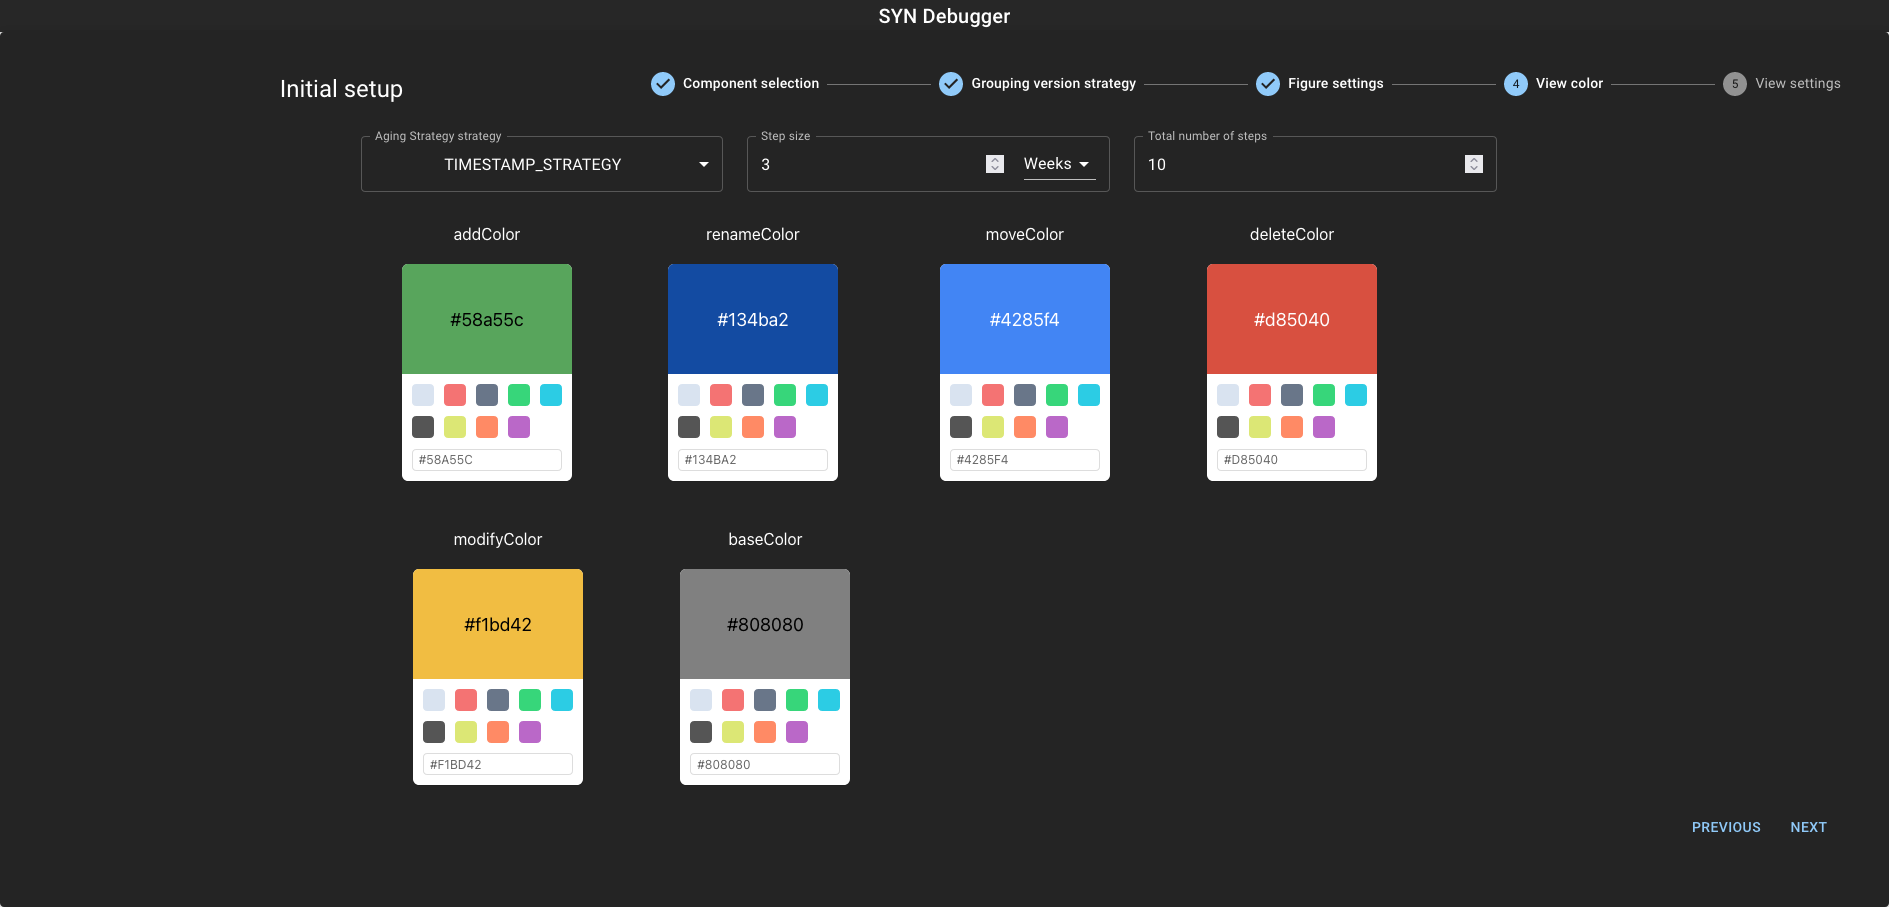
\includegraphics[width=\textwidth]{SYNUI-settings4.png}
    \caption{Project setup: view color}
    \label{fig:SYNUIsettings4}
\end{figure}

\subsubsection*{View settings}
The last step of the setup, shown in figure \ref{fig:SYNUIsettings5}, allows the user to express general preferences about the behaviour of the UI.

\begin{itemize}
    \item Show VR Button: if the UI should enable the full immersion experience that must be played with a VR headset. 
    \item Keep deleted entities: if the UI should keep deleted entities in the visualization. By default these are not displayed. 
    \item Show debug layer: if the debugger of the 3D engine should be visibile. 
    \item Auto screenshot: if a screenshot of the UI should be automatically done once the UI was rendered.
    \item Shadows: if the UI should compute and render shadows. 
    \item Animation switching speed: the amount of time between the render of one animation and another if the autoplay button is pressed. 
\end{itemize}

\begin{figure}
    \center
    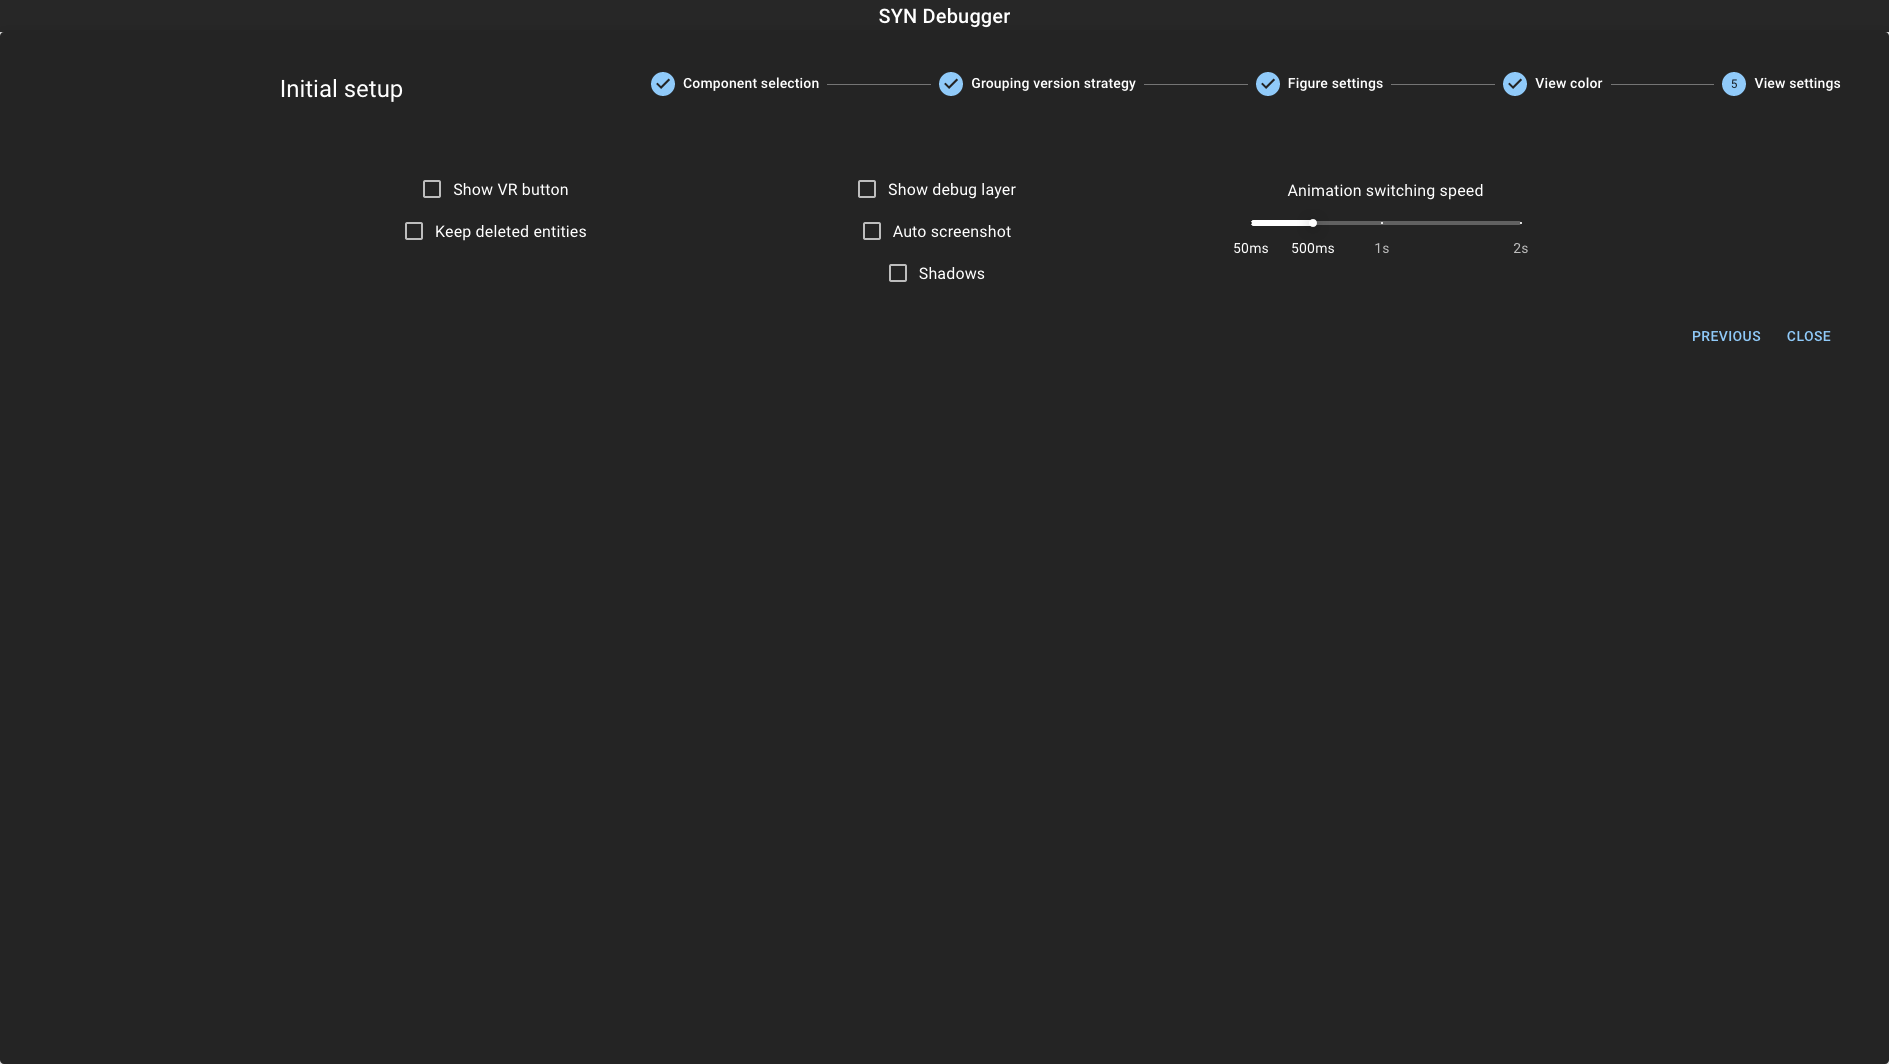
\includegraphics[width=\textwidth]{SYNUI-settings5.png}
    \caption{Project setup: view settings}
    \label{fig:SYNUIsettings5}
\end{figure}

\subsection*{Project visualization}
After having specified all the visualization preferences with the initial setup, all of them are stored in the local storage of the web browser. 
Therefore, the UI can retrieve, given the project id and the view specification, a view from the backend server. 

Initially it calls the partialView query provided by the SYN-Server module. Once it got the response, the visualization of the first AnimationFrame is automatically loaded. 
Since the partialView query returns only the first 100 AnimationFrames, to maximize the experience a prefetcher mechanisms was also implemented. 
Simply, once the half of the retrieved AnimationFrames have been displayed, it lazily requests a new partialView containing all the following AnimationFrames of the currently displayed view. 
In this way, the jump between a partialView and another is not subjected to network timing issues becuase the partial view was already prefetched before. 
\bigbreak

The initial display of the view is represented in figure \ref{fig:SYNUIsimple}. The visualization settings of this view are:
\begin{itemize}
    \item Version grouping strategy: timestamp, 3 weeks
    \item Color palette: default
    \item Aging: timestamp, 3 weeks with 10 steps
    \item Height mapper: BucketValueStrategy on SLOC
    \item Deleted entities are not shown
    \item All the entities have the same shape and opacity
    \item All the available metrics are selected for each FileType. 
\end{itemize}

The main visualization area can be broken down into four parts: 
In the box A we have a 3D environment displays FileHistories on a virtual plane. The camera is not fixed and with the mouse the view angle and the zoom level can be controlled. 
In the box B we have a card that depict the information about what the visualization is showing to the user. 
This card includes the tile of the project, the animation number displayed, the range of dates that this animationFrame has, a list of commits included inside this animation frame, a slider that shows the overall progress of the display, and two buttons to jump to the next or the previous animation, and finally one button to automatically jump to the next animation with the time interval previously set. 
Moreover, all the preferences specified during the project setup can be changed clicking on the three dots in the top right corner.
In the box C we have a card to inform the user on the number of entities that are rendered by the UI. 
And finally, box D appears only when an entity is selected with the mouse. 
It has: 
\begin{itemize}
    \item the name and the current path of the entity. The current path is the path of the entity on the last commit included in the displayed animation frame. 
    \item a table filled with all the metrics retrieved on the last commit of the displayed animation frame. The list of metrics is filtered with the one selected during the project setup. 
    \item a table filled with all the FileVersions associated to the selected FileHistory. Of each FileVersion the commit hash (clickable, it automatically redirects to github) and the action made on that commit is shown. Moreover, if with the mouse you hover on an action, a tooltip with commit information appears.
    \item a contextual menu shown if you right click on the card. With this contextual menu you can jump on github to see the raw file on the last commit of the current displayed animation. 
\end{itemize}

\begin{figure}
    \center
    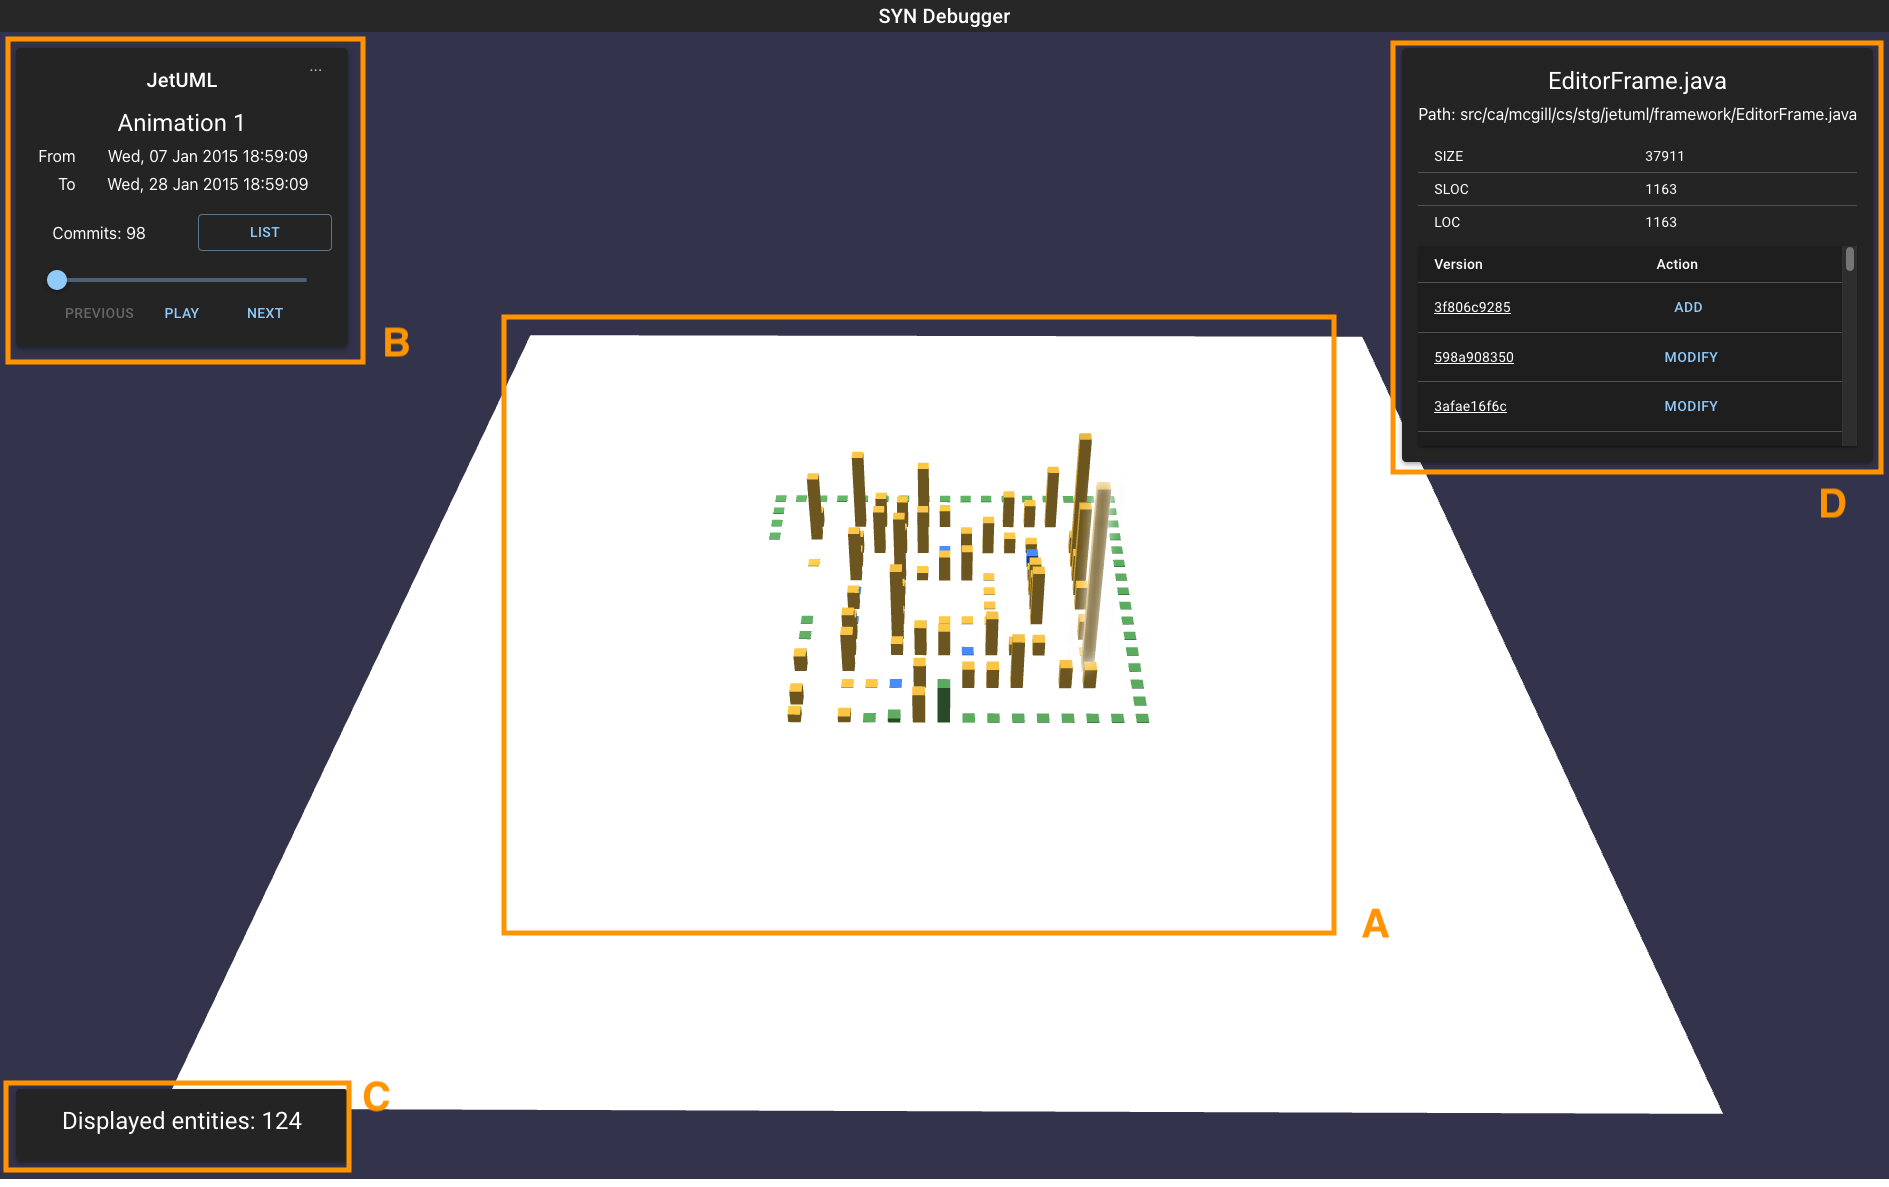
\includegraphics[width=\textwidth]{SYNUI-fileHistory.png}
    \caption{Visualization of JetUML with the default settings.}
    \label{fig:fileHistories}
\end{figure}

\begin{figure}
    \center
    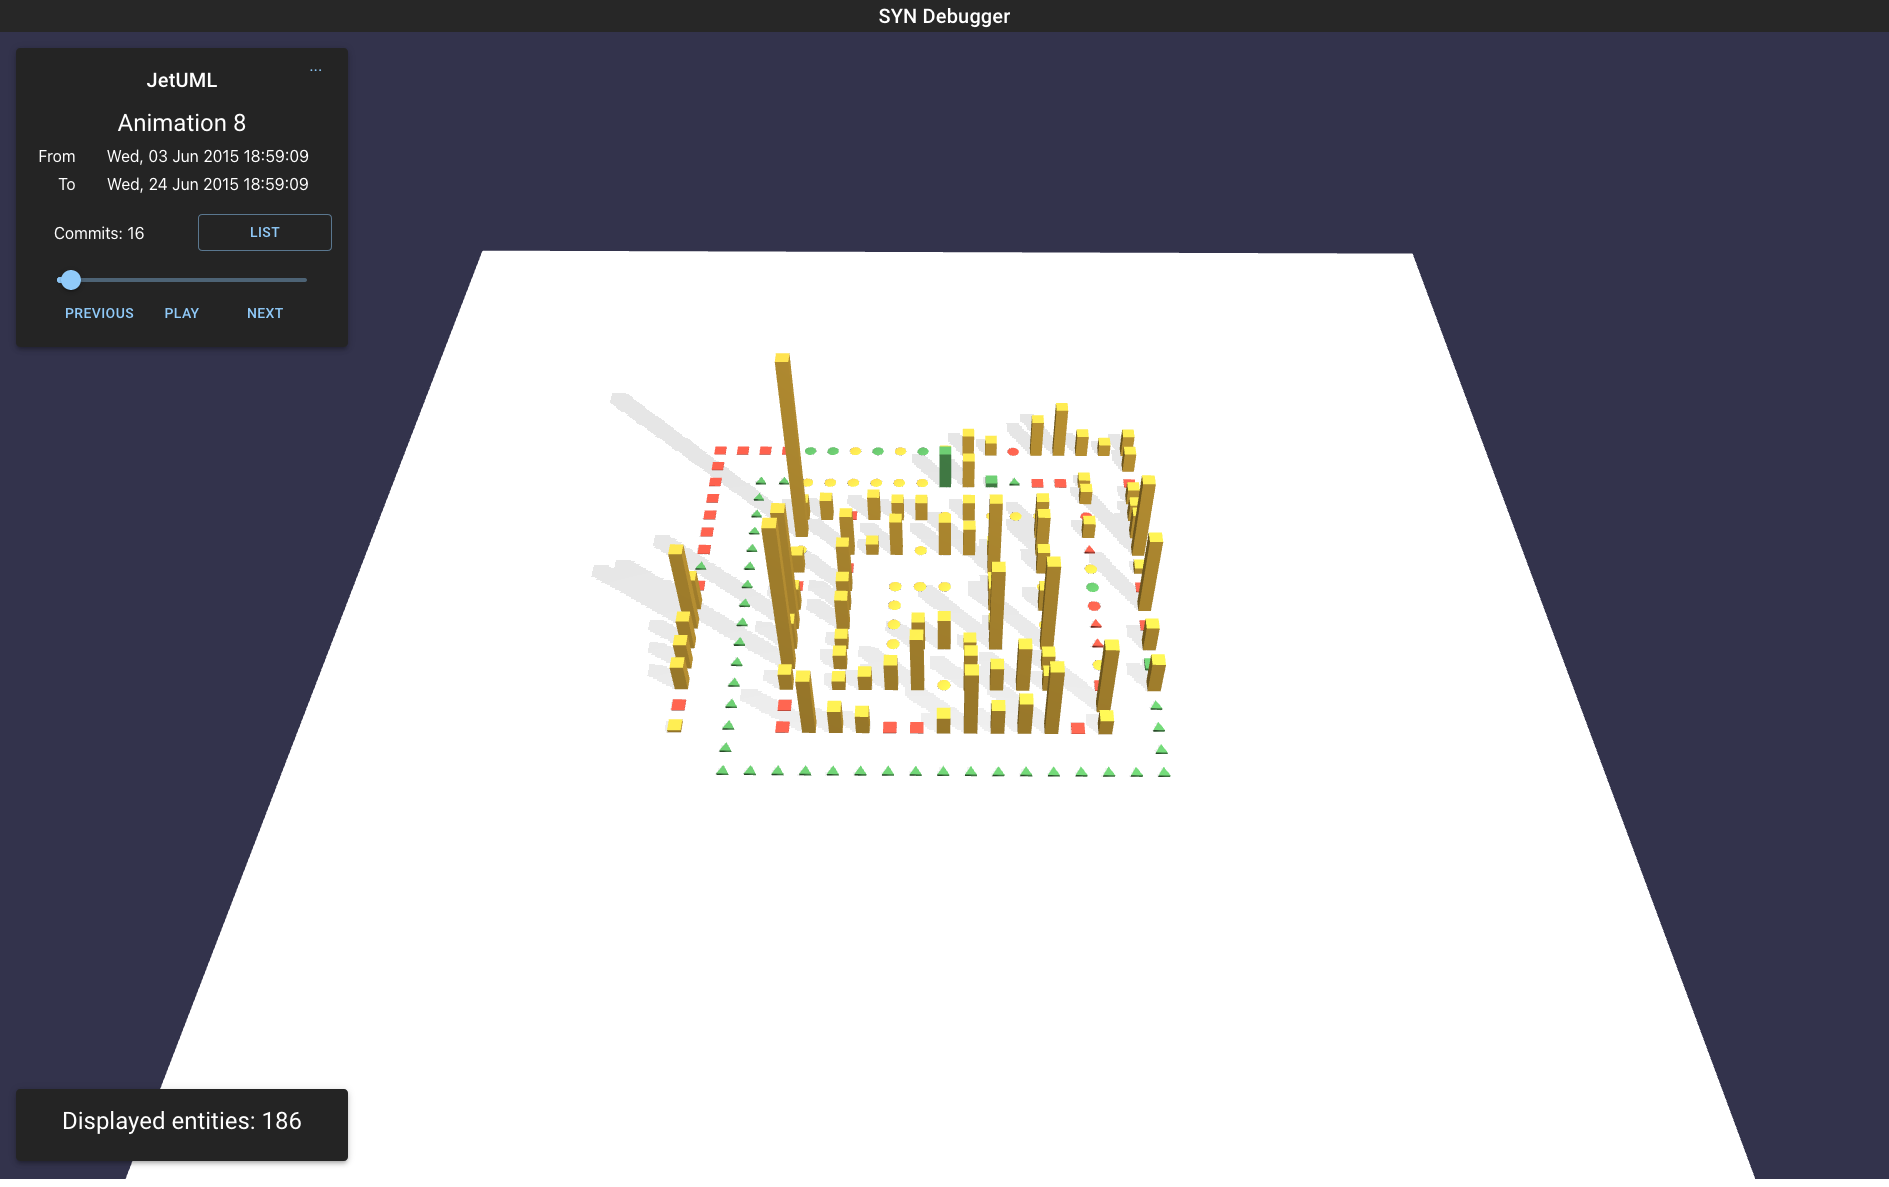
\includegraphics[width=\textwidth]{SYNUI-deletedshadow.png}
    \caption{Visualization of JetUML with shadows, deleted entities and custom shapes for non-java files.}
    \label{fig:deletedshadow}
\end{figure}